\begin{figure}[h]
    \centering
    \begin{subfigure}{.45\textwidth}
        \centering
        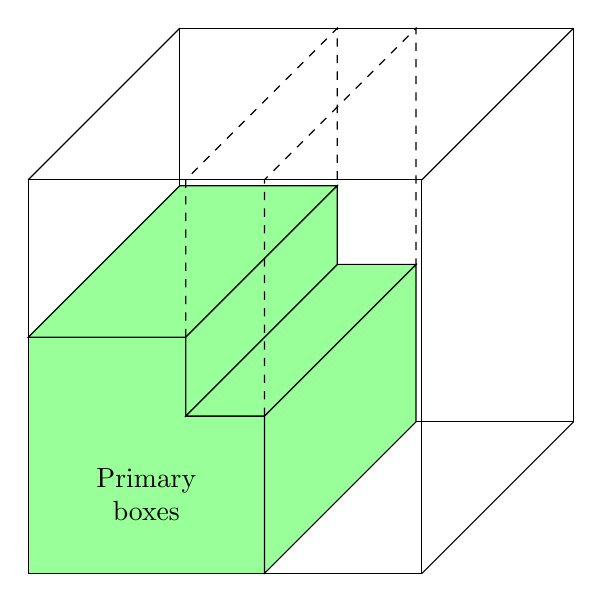
\begin{tikzpicture}[scale=0.5]
            \begin{scope}[fill=green!40]
                \draw (0,0,0) rectangle (10,10,0);
                \draw (0,0,-10) rectangle (10,10,-10);
                \draw (10,0,0) -- (10,0,-10);
                \draw (10,10,0) -- (10,10,-10);
                \draw (0,10,0) -- (0,10,-10);
                \filldraw (0,6,0) -- (0,6,-10) -- (4,6,-10) -- (4,6,0) -- cycle;
                \filldraw (0,0,0) -- (6,0,0) -- (6,4,0) -- (4,4,0) -- (4,6,0) -- (0,6,0) -- cycle;
                \filldraw (6,0,0) -- (6,0,-10) -- (6,4,-10) -- (6,4,0) -- cycle;
                \filldraw (6,4,0) -- (6,4,-10) -- (4,4,-10) -- (4,4,0) -- cycle;
                \filldraw (4,4,-10) -- (4,6,-10) -- (4,6,0) -- (4,4,0) -- cycle;
                \draw[dashed] (4,6,0) -- (4,10,0) -- (4,10,-10) -- (4,6,-10);
                \draw[dashed] (6,4,0) -- (6,10,0) -- (6,10,-10) -- (6,4,-10);
                \node[align=center] at (3,2) {Primary\\boxes};
            \end{scope}
        \end{tikzpicture}
        \caption{}
        \label{fig:remaining spaces first filling WBH A}
    \end{subfigure}
    \begin{subfigure}{.45\textwidth}
        \centering
        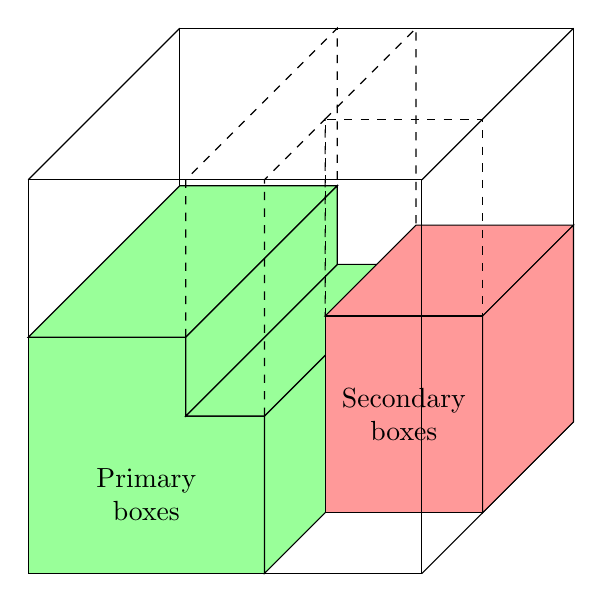
\begin{tikzpicture}[scale=0.5]
            \begin{scope}[fill=green!40]
                \draw (0,0,0) rectangle (10,10,0);
                \draw (0,0,-10) rectangle (10,10,-10);
                \draw (10,0,0) -- (10,0,-10);
                \draw (10,10,0) -- (10,10,-10);
                \draw (0,10,0) -- (0,10,-10);
                \filldraw (0,6,0) -- (0,6,-10) -- (4,6,-10) -- (4,6,0) -- cycle;
                \filldraw (0,0,0) -- (6,0,0) -- (6,4,0) -- (4,4,0) -- (4,6,0) -- (0,6,0) -- cycle;
                \filldraw (6,0,0) -- (6,0,-10) -- (6,4,-10) -- (6,4,0) -- cycle;
                \filldraw (6,4,0) -- (6,4,-10) -- (4,4,-10) -- (4,4,0) -- cycle;
                \filldraw (4,4,-10) -- (4,6,-10) -- (4,6,0) -- (4,4,0) -- cycle;
                \node[align=center] at (3,2) {Primary\\boxes};
            \end{scope}
            \begin{scope}[fill=red!40]
                \filldraw (6,5,-4) -- (6,5,-10) -- (10,5,-10) -- (10,5,-4) -- cycle;
                \filldraw (10,0,-4) -- (10,0,-10) -- (10,5,-10) -- (10,5,-4) -- cycle;
                \filldraw (6,0,-4) -- (10,0,-4) -- (10,5,-4) -- (6,5,-4) -- cycle;
                \draw (10,0,0) -- (10,10,0);
                \draw[dashed] (6,5,-4) -- (6,10,-4) -- (10,10,-4) -- (10,5,-4);
                \draw[dashed] (6,10,-4) -- (6,10,-10) -- (6,5,-10);
                \draw[dashed] (6,4,0) -- (6,10,0) -- (6,10,-4) -- (6,5,-4);
                \draw[dashed] (4,6,0) -- (4,10,0) -- (4,10,-10) -- (4,6,-10);
                \node[align=center] at (8,2.5,-4) {Secondary\\boxes};
            \end{scope}
        \end{tikzpicture}
        \caption{}
        \label{fig:remaining spaces first filling WBH B}
    \end{subfigure}
    \caption{Remaining spaces in the first filling of a layer}
    \label{fig:remaining spaces first filling WBH}
\end{figure}